\section{Reinforcement learning}

In the realm of artificial intelligence, learning methods can be categorized into three types: supervised learning, unsupervised learning, and reinforcement learning, each having its own uses and advantages.

\textbf{Supervised learning} learns from a labelled dataset, where each input has a corresponding desired output. The goal is generalize and make accurate predictions for new, unseen data. This method is commonly used for regression and classification tasks, where the algorithm iteratively adjusts its parameters to minimize the difference between predicted and true values. Accuracy of predictions is heavily dependent of quality of dataset.

\textbf{Unsupervised learning} learns on unlabelled datasets. It discovers inherent patterns or structures within the data. Common tasks include clustering similar data points or reducing dataset dimensionality. Unsupervised learning is used for exploring large datasets, uncovering hidden relationships, and helping in data visualization.

\textbf{Reinforcement learning} learns from interaction with environment through actions and rewards. Its goal is mapping environment states to actions order to maximize long term reward. It is used in robotics, self-driving cars or playing games. One of main characteristics is trial and error.

\begin{figure}
\label{multiNet}
\centering
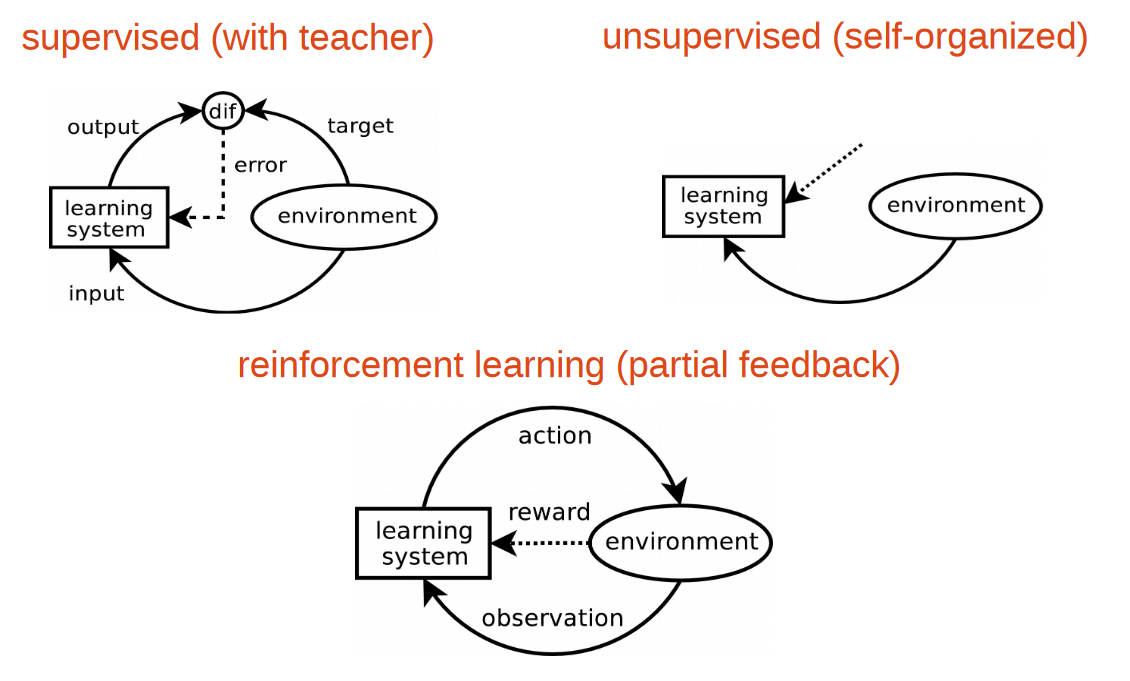
\includegraphics[width=0.9\textwidth]{images/rl.png}
\caption{Different categories of AI learning methods \cite{NNFarkas}}
\end{figure}

\subsubsection{Introduction}